%%%%%%%%%%%%%%%%%%%%%%%%%%%%%%%%%%%%%%%%%%%%%%%%%%%%
% This will help you in writing your homebook
% Remember that the character % is a comment in latex
%
% chapter 1
\chapter{Protocol}
\label{chap1}

%%%%%%%%%%%%%%%%%%%%%%%%%%%%%%%%%%%%%%%%%%%%%%%%%%%%%%%%%%%
% you can organize a chapter using sections -> \section{Simulating an inverter}
% or subsections -> \subsection{simulating a particular type of inverter}

%%%%%%   First section

\section{Read Transaction}

Whenever the CPU wants to begin a transaction with one of the IPs present on the FPGA, it writes at address 0 of the buffer a data packet compliant with the following specifications: 
\bigskip
\begin{center}
	\begin{tabular}{ | l | l |  l | l | l |}
		
		15 & 14 & 13 & 12 & 11 \qquad \qquad 0 \\ \hline
		R/W & INT & B/E & UNUSED & IP ADDR\\ \hline
		
		
		\hline
	\end{tabular}
\end{center}

\bigskip
\begin{center}
	\begin{tabular}{ | c | p{7 cm} |  l |}
		\hline
		Bit(s) & Purpose & Value(s)  \\ \hline
		Bit 15 & It specifies whether the transaction is a read or write transaction.  & Read = 0, Write = 1 
		 \\ \hline

		Bit 14 & Specifies whether the current transaction is due to an interrupt request   & Normal = 0, Interrupt  =  1
		\\ \hline
		
		Bit 13 & Signals the begin/end of a transaction & Begin  = 1, End = 0 
			\\ \hline
		Bit 12 & Unused & Unused 	
			
				\\ \hline		
				Bit 11-0 & The physical address of the target IP (in general is different form the IP number) &
				From 0 up to N-1  \\
		 
		
		
		\hline
	\end{tabular}
\end{center}
\bigskip
The various step for a read operations are:\\
\begin{enumerate}
	\item \textbf{Control word for the IP manager}\\
	 The CPU writes at address 0 the control word for the IP manager.
	 For example it could write
	 
	 \begin{center}
	 	\begin{tabular}{ | l | l |  l | l | l |}
	 		
	 		15 & 14 & 13 & 12 & 11 \qquad \qquad 0 \\ \hline
	 		R/W & INT & B/E & UNUSED & IP ADDR\\ \hline
				0 & 0 & 1 & * & 000000000000\\ \hline	 		
	 		
	 		\hline
	 	\end{tabular}
	 \end{center}
	
	 \bigskip
	 Then the buffer will give this data to the IP CORE manager (\textit{row\_0})
	 
	 \item \textbf{IP manager will activate the transaction}\\
	 The IP manager will enable the selected IP Core and give the right input to the switch.
	 
	 \item \textbf{IP core gives the data}\\
	 The selected IP core will write some data to the buffer, thus the CPU can now read the value of the IP CORE from the buffer.
	 
	 \item \textbf{Close transaction}\\
	 The CPU writes at address 0 the control word for the IP manager to close the transaction.
	 In this case it will disable all the IP Cores.
	 
	 \begin{center}
	 	\begin{tabular}{ | l | l |  l | l | l |}
	 		
	 		15 & 14 & 13 & 12 & 11 \qquad \qquad 0 \\ \hline
	 		R/W & INT & B/E & UNUSED & IP ADDR\\ \hline
	 		0 & 0 & 0 & * & 000000000000\\ \hline	 		
	 		
	 		\hline
	 	\end{tabular}
	 \end{center}
	 
\end{enumerate}
% Below is shown how you can insert a figure. If you give a label to the figure, you can refer to the figure using \ref{figure_label} as shown above. 
\bigskip
\bigskip

 \begin{figure}[h]
 	\centering
 	\includegraphics[scale=0.75]{chapters/figures/read_0.png}  
 	\caption{\textbf{Write the control signal on address 0 of the buffer.} \\Since the buffer is asynchronous, it will give this info to the IP Manager as soon as possible with the signal \textit{row\_0}}
 	\label{fig:0}
 \end{figure}
 
  \begin{figure}[h]
  	\centering
  	\includegraphics[scale=0.75]{chapters/figures/read_1.png}  
  	\caption{\textbf{IP Manager activate the transaction}. \\The IP Manager will enable the selected IP on the falling edge of the clock. The selected IP will do nothing because it is positive edge sensitive. In the meantime the IP Manager will give the right value to the switch. Even if the switch is active, both the buffer and the IP\_0 are uneffected: \textit{w\_ip\_to\_buffer} and\textit{ Write} to the IP signals are '0'}
  	\label{fig:1}
  \end{figure}
  
   \begin{figure}[h]
   	\centering
   	\includegraphics[scale=0.75]{chapters/figures/read_2.png}  
   	\caption{\textbf{IP core gives the data.} \\
   		Now that we have the rising edge of the clock, the IP core is active, and will give the data to the switch which will forward it to the buffer. Both the switch and the Buffer are always active (asynchronous). That means that the CPU can ask the buffer to read the new value.\\\\
   		If there were any problems (e.g. latency), the CPU can ask the buffer to read in this clock cycle and check tha value on the \textit{Data} signal on the next clock cycle.}
   	\label{fig:2}
   \end{figure}
   
    \begin{figure}[h]
    	\centering
    	\includegraphics[scale=0.75]{chapters/figures/read_3.png}  
    	\caption{\textbf{Close transaction}\\ The CPU has to tell to the IP Manager to disable all the IP Core \textit{row\_0}}
    	\label{fig:3}
    \end{figure}
    
     \begin{figure}[h]
     	\centering
     	\includegraphics[scale=0.75]{chapters/figures/read_4.png}  
     	\caption{\textbf{Transaction closed}\\ IP manager disables the IP core}
     	\label{fig:4}
     \end{figure}
